\documentclass[../../../../dd.tex]{subfiles}

\begin{document}

	\section{Deployment View}
		\href{https://en.wikipedia.org/wiki/Deployment_diagram}{descrizione}
		
		The main hardware devices involved in this system are the following:
		\begin{itemize} 
		\item Web Server: on this server we have the logic tier of our application, this tier contain the logical part of the system, so this devices must have the higher computation power between the devices. It offer via HTTP the connection from the user, and access to the database via XMPP ( communication protocol based on XML typical used for inter-server communication).
		\item Data Base Server: on this server we have the data tier of our application. This device must store on its memory all the data of our system. So, to avoid problem, the memory of this device must be suitable for store all the information. This device must be connected to the web server for the purpose of make available to the logic tier the information that the data tier store. the communication between this two takes place in XMPP.
		\item User Devices: this kind of devices are divided into Mobile Devices and Computers. On this kind of devices we have the presentation tier of our application. The kind of component we use on this devices depends on the type of devices and the OS installed (as we have described on the chapter Software Limitation in the RASD) . We can't know the hardware specification of this devices so the presentation tier must be lighter as possible.  the communication between this devices and the Web Server takes place in HTTP between the internet.
	\end{itemize}
	
	
	\begin{figure}[H]
				\centering
				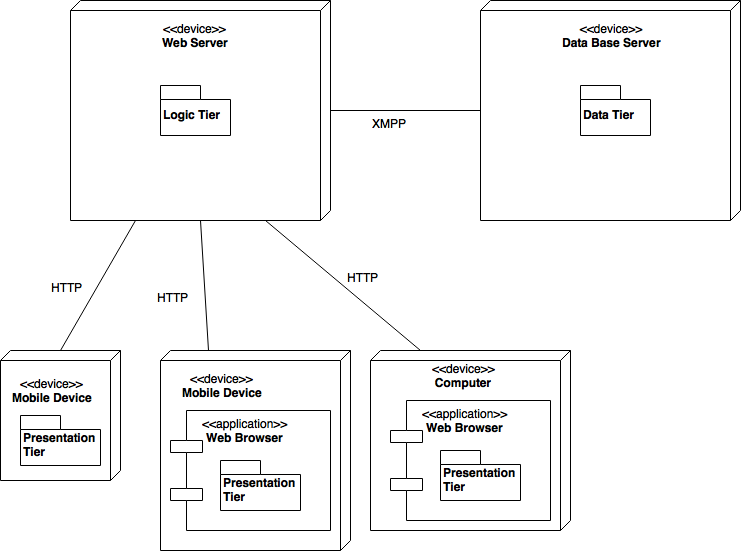
\includegraphics[width=\textwidth, scale=0.5]{../images/Deploy.png}
			\caption{Deployment Diagram}\label{fig:Deploy}
		\end{figure}
	
\end{document}